\section{Struttura del sorgente Android}
\begin{figure}[thp]
\centering
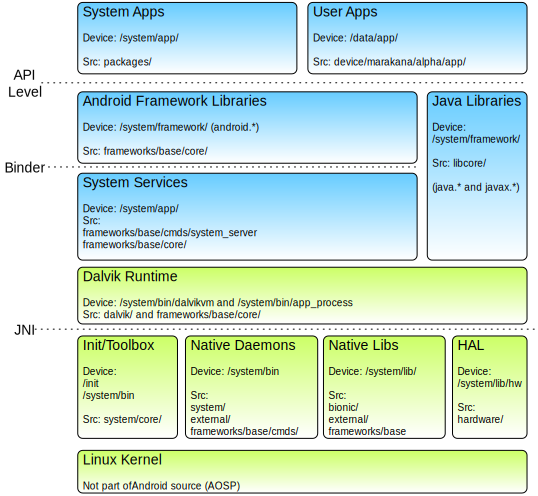
\includegraphics[scale=0.7]{img/marak/asstd}
\caption{Visualizzazione dell'Architettura di Android dal punto di vista dei 
Device e dei sorgenti. \parencite{site:marakRemixing}}
\label{fig:androidsourceView}
\end{figure}
Possiamo avvicinarci alla struttura dei sorgenti Android guardando alla Figura
\vref{fig:androidsourceView}: come possiamo vedere, la parte del Kernel Android
non è inclusa all'interno del sorgente AOSP di Android, che contiene unicamente 
i sorgenti per l'\textit{Android Middleware}. É sempre possibile reperire
la versione del Kernel più appropriata al dispositivo, scegliendo tra le seguenti
varianti (\texttt{\small\d PATH}); tra le più rappresentative:
\begin{description}
\item[kernel/common]   è il branch ufficiale del Kernel Linux, che viene utilizzato come base per tutte le altre versioni seguenti.
\item[kernel/goldfish] Kernel \textit{tree} da utilizzare per ottenere le immagini Kernel per l'architettura dell'emulatore, detta appunto ``Goldfish''.
\item[kernel/msm] Kernel \textit{tree} da utilizzare per i Chipset Qualcomm, tra i quali annoveriamo il Nexus One \parencite{tesi:nexus}.
\item[kernel/samsung]  Kernel \textit{tree} per i sistemi Samsung.
\item[kernel/tegra]    Kernel \textit{tree} per i chipset Tegra.
\end{description}

Per scaricare tali versioni del kernel, è sufficiente postporre i percorsi di cui
sopra al seguente comando:
\begin{center}
\texttt{\small git clone https://android.googlesource.com/\d PATH}
\end{center}
Ricordo che, dopo aver effettuato il \texttt{\small clone} sul \textit{repository}, è possibile
visualizzarne i branch remoti tramite il comando \texttt{git branch -a}, e quindi 
effettuare il \texttt{\small checkout} dei files per poterli visualizzare sul 
computer locale:
\begin{center}
\texttt{\small git checkout remotebranchpath}
\end{center}
\medskip

Tuttavia non è nell'interesse di questa tesi descrivere in un modo più approfondito quale
sia la struttura dei sorgenti del Kernel, in quanto mi concentrerò maggiormente
sull'\textit{AOSP Source}, il quale ci permetterà di generare il \textit{ramdisk} alla
fine di effettuare il \textit{flashing} sul dispositivo Galaxy Nexus. 
Andando ora ad analizzare la struttura dello AOSP Source, possiamo identificare
i seguenti \textit{folder} principali:

\begin{description}
\item[bionic] Contiene la libreria Bionic per il supporto della \textit{libc}; di questa si parlerà nella Sezione \vref{sec:diffbilib}.
\item[bootable] Contiene il supporto a \textit{bootloader}, \textit{diskinstaller}, e al \textit{recovery image}.
\item[build] Contiene gli script di supporto alla compilazione.
\item[cts] Contiene la  \textsc{Android’s Compatibility Test Suite}, allo scopo di effettuare dei testing sul sorgente.
\item[dalvik] Contiene la definizione della \textsc{Dalvik Virtual Machine} (DVM).
\item[development] Contiene \textit{tool} per lo sviluppo, file di configurazione ed applicazioni d'esempio.
\item[device] Contiene binari e sorgenti specifici per il dispositivo sul quale portare l'AOSP Source.
\item[external] Contiene le librerie native e Java di terze parti, ottenute tramite il la sincronizzazione con \textit{repository} remoti.
\item[frameworks] \label{sec:explainframe} Contiene utilità native per Android, demoni (\texttt {installd}, \\
\texttt{servicemanager}, \texttt{system\_server}), l'utilizzo di librerie (quali quelle di supporto all'architettura tramite \textit{wrapper} JNI), l'implementazione delle API Android e dei \texttt{services}. 
\item[hardware] Fornisce le librerie di supporto all'astrazione dello hardware (HAL - \textsc{Hardware Abstraction Layer}), fornendo alcuni sorgenti ed oggetti binari.
\item[ndk] v. Sezione \vref{sec:NDKtool}
\item[out] Contiene il risultato del processo di compilazione
\item[packages] Contiene le applicazioni e le utility di sistema comuni a tutti i dispositivi Android commercializzati.
\item[prebuilt] Contiene binari precompilati, quali kernel ed altri binari di terze parti.
\item[sdk] Contiene i tool per l'Android SDK (v. Sezione \vref{sec:SDKStep}).
\item[system] Contiene la \textit{root} del FileSystem di Android, alcuni ``demoni nativi``, la definizione di \texttt{\small init} ed i file di configurazione.    
\end{description}

Identificherò la cartella che contiene tali \textit{folder} come \AOSP.
 
\subsection{AOSP: Configurazione dell'ambiente ed ottenimento dei sorgenti}
Per la compilazione di questo sorgente non è necessario fornire, come nel caso 
della compilazione del kernel,  un \textit{crosscompiler}, in quanto questo verrà generato
automaticamente dalla compilazione tramite i sorgenti messi a disposizione. Per
rendere possibile la compilazione degli \textit{host tool} forniti nel sorgente, è 
necessario effettuare l'installazione dei seguenti pacchetti:
\begin{bash}
sudo apt-get install git-core gnupg flex bison gperf build-essential \
  zip curl libc6-dev libncurses5-dev:i386 x11proto-core-dev \
  libx11-dev:i386 libreadline6-dev:i386 libgl1-mesa-glx:i386 \
  libgl1-mesa-dev g++-multilib mingw32 openjdk-6-jdk tofrodos \
  python-markdown libxml2-utils xsltproc zlib1g-dev:i386
\end{bash}
Per risolvere inoltre un problema nella compilazione, è necessario effettuare il
seguente \textit{link}:
\begin{bash}
sudo ln -s /usr/lib/i386-linux-gnu/mesa/libGL.so.1 /usr/lib/i386-linux-gnu/libGL.so
\end{bash}

Per quanto concerne invece il compilatore di Java, non si garantisce la corretta 
compilazione dei sorgenti tramite l'utilizzo di \texttt{IcedTea} per \texttt{OpenJDK},
implementazione GNU GPL del linguaggio Java: è necessario pertanto scaricare 
i binari ufficiali di Oracle al seguente indirizzo:
\begin{center}
\small
\url{http://www.oracle.com/technetwork/java/javase/downloads/jdk6-downloads-1637591.html}
\end{center}

Se il proprio sistema supporta già un'implementazione Open di Java, sarà successivamente
necessario eseguire questi comandi allo scopo di utilizzare la versione standard
scaricata dall'indirizzo di cui sopra:
\begin{bash}
sudo update-alternatives --install /usr/bin/java java /usr/lib/jvm/jdk1.6.0_33/bin/java 1
sudo update-alternatives --install /usr/bin/javac javac /usr/lib/jvm/jdk1.6.0_33/bin/javac 1
sudo update-alternatives --install /usr/bin/javaws javaws /usr/lib/jvm/jdk1.6.0_33/bin/javaws 1
sudo update-alternatives --config java
sudo update-alternatives --config javac
sudo update-alternatives --config javaws
\end{bash}
Per evitare ulteriori e possibili problemi in fase di compilazione, come ad 
esempio \textit{Could not stat out/target/product/generic/system}, ovvero l'assenza della cartella
ove vengono immessi i binari dai quali produrre poi l'immagine del \textit{filesystem}
di sistema, è opportuno installare i seguenti programmi.
\begin{bash}
sudo apt-get install xmlto doxygen
\end{bash}
\medskip

Per poter scaricare il sorgente AOSP completo, si rivela necessario utilizzare
lo script \texttt{\small repo}, reso disponibile dalla stessa Google all'indirizzo
\begin{center}
\small
\url{https://dl-ssl.google.com/dl/googlesource/git-repo/repo}
\end{center}

Per scaricare l'ultima versione del sorgente, è  sufficiente
eseguire i comandi che seguono da terminale all'interno della cartella \AOSP; mentre il primo permette l'inizializzazione
del \textit{repository}, il secondo permette il \textit{download} effettivo dell'intero
sorgente.
\begin{bash}
repo init -u https://android.googlesource.com/platform/manifest
repo sync
\end{bash}
\medskip

Leggendo sul sito attinente alla documentazione ufficiale sui sorgenti Android,
\url{http://sources.android.com}, si osserva la seguente nota informativa:
\begin{quotation}
\textit{
Starting with Ice Cream Sandwich, the Android Open-Source Project can't be used from pure source code only, and requires additional hardware-related proprietary libraries to run, specifically for hardware graphics acceleration.
}
\end{quotation}
\begin{quotation}
\textit{
Each set of binaries comes as a self-extracting script in a compressed archive. After uncompressing each archive, run the included self-extracting script from the root of the source tree, confirm that you agree to the terms of the enclosed license agreement, and the binaries and their matching makefiles will get installed in the vendor/ hierarchy of the source tree.
}
\end{quotation}
Per quanto concerne i telefoni riconosciuti da Google come Developer Phones, è
possibile scaricare gli script a loro dedicati tramite il sito:
\begin{center}
\url{https://developers.google.com/android/nexus/drivers}
\end{center}
Tuttavia, anche in questo modo non vengono forniti tutti i driver atti ad un utilizzo
completo del dispositivo\footnote{v. \url{http://source.android.com/source/known-issues.html}}:
\begin{quotation}
\textit{Camera, GPS and NFC don't work on Galaxy Nexus.}
\end{quotation}
\begin{quotation}
\textit{Symptom: Camera, GPS and NFC don't work on Galaxy Nexus. As an example, the Camera application crashes as soon as it's launched.}
\end{quotation}
\begin{quotation}
\textit{Cause: Those hardware peripherals require proprietary libraries that aren't available in the Android Open Source Project.}
\end{quotation}
\begin{quotation}
\textit{Fix: None.}
\end{quotation}
Per altri dispositivi, quali il Samsung Galaxy SIII, è la stessa Samsing a rilasciare
i sorgenti all'indirizzo \url{http://opensource.samsung.com}.

\subsection{AOSP: compilazione dei sorgenti e \textit{flashing} del dispositivo.}\label{subsec:compileaosp}
Dopo la procedura di configurazione e di ottenimento dei sorgenti, è possibile
procedere con la loro compilazione. Per assicurarsi in ogni momento che la 
cartella di \textit{output} sia effettivamente pulita, è possibile 
eseguire il comando:
\begin{center}
\texttt{\small make clobber}
\end{center}
Devo però avvertire a questo punto che questa operazione cancella completamente
le configurazioni precedenti. Pertanto è opportuno eseguire di nuovo
la procedura di configurazione come illustrato di seguito.
Per iniziare la creazione dell'ambiente di cross-compilazione, è opportuno
eseguire il comando:
\begin{center}
\texttt{\small . build/envsetup.sh}
\end{center}
Successivamente, fornendo il comando \texttt{\small lunch}, si può scegliere per
quale dispositivo effettuare la compilazione. Nel
caso specifico del dispositivo Galaxy Nexus oggetto di Tesi, ho preferito utilizzare
la configurazione \texttt{\small full\_maguro-userdebug}, in quanto \texttt{\small full}
indica la compilazione completa del sorgente, \texttt{\small maguro} è il \textit{codename}
del dispositivo e \texttt{\small userdebug} consente la visualizzazione di maggiori
stampe a video di debug tramite LogCat, assieme all'attivazione dei permessi di
root di default. In seguito lanciando il comando
\begin{center}
\texttt{\small make -jn}
\end{center}
si avvia la compilazione, dove in particolare \texttt{\small n} identifica il numero
di processi desiderati per effettuare la compilazione, terminata la quale
si otterrà l'immagine prodotta all'interno del percorso \texttt{\small \d ANDROID/out/target/product/generic}.
Se questa non fosse sufficiente per la generazione del file (es.) \texttt{\small
system.img}, un secondo processo di compilazione dovrebbe portare alla loro 
corretta compilazione.
\medskip

Per proseguire ora con la procedura di \textit{flashing} della \textit{custom image},
è opportuno dichiarare in prima istanza una variabile globale \texttt{\small ANDROID\_PRODUCT\_OUT}
con la quale definire quale sia il percorso contentente le immagini di sistema,
tramite le quali consentire l'operazione di \textit{flashing}, ed opzionalmente indicare
quale sia il percorso dove sono stati compilati i binari per effettuare l'interazione
con i dispositivi\footnote{Questi binari sono tuttavia gli stessi proposti
all'interno dell'SDK di Google.}.
\begin{bash}
export PATH=\$AOSP/out/host/linux-x86/bin:\$PATH
export ANDROID_PRODUCT_OUT=\$AOSP/out/target/product/maguro
cd \$ANDROID_PRODUCT_OUT
\end{bash}
Prima di effettuare l'operazione di flashing, è opportuno effettuare un 
backup del dispositivo, come illustrato nella Sottosezione \vref{subsec:rootingn},
allo scopo di poter ripristinare in un secondo momento le configurazioni
precedenti del dispositivo e le applicazioni Java installate. Per proseguire
con il \textit{flashing} è tra l'altro necessario effettuare l'\textit{unlocking} del
dispositivo ed in seguito accedere alla modalità \textit{bootloader}, come tra l'altro
già illustrato in quella Sottosezione per il Samsung Galaxy Nexus.

Per inviare le immagini prodotte all'interno del dispositivo, sarà sufficiente
eseguire il seguente comando:
\begin{bash}
fastboot -w flashall
\end{bash}
L'operazione di flashing verrà avviata solamente se tutti i file(s) necessari
saranno stati prodotti dalla precedente compilazione: in questo modo non si 
rischia di effettuare un'operazione parzialmente corretta.
